% F035 指数幂的运算法则｜04 例题：从会算到会选最快方法
\begin{examplebox}
    \textbf{\textcolor{CExample}{例1｜基础：先看底数有没有变}}\par
    \textbf{题目：} 计算 $2^3\cdot2^4$。\par
    \textbf{最快思路：} 底数都是 $2$，连乘时指数相加。
    \[2^3\cdot2^4=2^{3+4}=\boxed{2^7=128}.\]
    \begin{center}
    \begin{tikzpicture}[font=\small,>=stealth]
        \node[draw=blue!55,fill=blue!7,rounded corners=3pt] (a) at (0,0) {3 个 $2$};
        \node[draw=blue!55,fill=blue!7,rounded corners=3pt] (b) at (3.2,0) {4 个 $2$};
        \node at (1.6,0) {$+$};
        \node[draw=green!50!black,fill=green!10,rounded corners=3pt,inner sep=5pt] (c) at (1.6,-1.2) {$2^{3+4}=2^7$};
        \draw[->,thick] (1.6,-0.35)--(c.north);
    \end{tikzpicture}

    \end{center}
    \textbf{记住：} 这里相加的是\textbf{指数}，不是把两个幂的值相加。
\end{examplebox}

\begin{examplebox}
    \textbf{\textcolor{CExample}{例2｜连用三条法则：先括号，后合并}}\par
    \textbf{题目：} 化简 $(3x^2)^3\cdot x^4$（$x>0$）。\par
    \textbf{步骤1：} 积的乘方，$3$ 和 $x^2$ 都要乘方。\par
    \textbf{步骤2：} 幂的乘方，指数相乘；最后同底相乘，指数相加。
    \[
      \begin{aligned}
        (3x^2)^3\cdot x^4
        &=3^3(x^2)^3\cdot x^4\\
        &=27x^{2\times3}\cdot x^4\\
        &=\boxed{27x^{6+4}=27x^{10}}.
      \end{aligned}
    \]
    \begin{center}
    \begin{tikzpicture}[font=\small,>=stealth]
        \node[draw=orange!65,fill=orange!7,rounded corners=3pt,inner sep=5pt] (a) at (0,0) {$(3x^2)^3$};
        \node[draw=blue!55,fill=blue!7,rounded corners=3pt,inner sep=5pt] (b) at (3.7,0) {$3^3\cdot x^6$};
        \node[draw=green!55!black,fill=green!10,rounded corners=3pt,inner sep=5pt] (c) at (7.2,0) {$27x^{10}$};
        \draw[->,thick] (a.east)--node[above,font=\footnotesize]{分开乘方}(b.west);
        \draw[->,thick] (b.east)--node[above,font=\footnotesize]{再乘 $x^4$}(c.west);
    \end{tikzpicture}

    \end{center}
    \textbf{记住：} 括号里的 $3$ 也有三次方，不能漏成 $3x^6$。
\end{examplebox}

\begin{examplebox}
    \textbf{\textcolor{CExample}{例3｜指数方程：先化成相同底数}}\par
    \textbf{题目：} 解 $4^x\cdot2^{x+1}=32$。\par
    \textbf{为什么这么想：} $4=2^2$，$32=2^5$，统一写成底数 $2$ 最快。
    \[
      \begin{aligned}
        (2^2)^x\cdot2^{x+1}&=2^5,\\
        2^{2x+x+1}&=2^5,\\
        3x+1&=5,\\
        x&=\boxed{\frac43}.
      \end{aligned}
    \]
    因为底数 $2>0$ 且 $2\ne1$，相同底数的两个幂相等时，指数相等。
    \begin{center}
    \begin{tikzpicture}[font=\small,>=stealth]
        \node[draw=orange!60,fill=orange!7,rounded corners=3pt,inner sep=5pt] (a) at (0,0) {$4^x\cdot2^{x+1}=32$};
        \node[draw=blue!60,fill=blue!7,rounded corners=3pt,inner sep=5pt] (b) at (4.5,0) {$2^{3x+1}=2^5$};
        \node[draw=green!60!black,fill=green!10,rounded corners=3pt,inner sep=5pt] (c) at (8.0,0) {$x=\frac43$};
        \draw[->,thick] (a.east)--node[above,font=\footnotesize]{化同底}(b.west);
        \draw[->,thick] (b.east)--node[above,font=\footnotesize]{比指数}(c.west);
    \end{tikzpicture}

    \end{center}
    \textbf{记住：} 底数若为 $1$，不能靠“指数相等”解方程。
\end{examplebox}

\begin{examplebox}
    \textbf{\textcolor{CExample}{例4｜零、负数和分数指数：先认清含义}}\par
    \textbf{题目：} 计算 $16^{1/2}\cdot2^{-1}+5^0$。\par
    \textbf{最快思路：} $16^{1/2}$ 是 $\sqrt{16}$，$2^{-1}$ 是 $1/2$，$5^0=1$。
    \[16^{1/2}\cdot2^{-1}+5^0=4\cdot\frac12+1=\boxed{3}.\]
    \begin{center}
    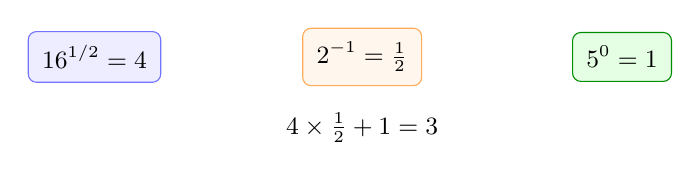
\begin{tikzpicture}[font=\small]
        \node[draw=blue!55,fill=blue!7,rounded corners=3pt,inner sep=5pt] at (0,0) {$16^{1/2}=4$};
        \node[draw=orange!65,fill=orange!7,rounded corners=3pt,inner sep=5pt] at (3.4,0) {$2^{-1}=\frac12$};
        \node[draw=green!55!black,fill=green!10,rounded corners=3pt,inner sep=5pt] at (6.7,0) {$5^0=1$};
        \node at (3.4,-0.9) {$4\times\frac12+1=3$};
    \end{tikzpicture}

    \end{center}
    \textbf{记住：} 负指数不是算出负数，分数指数也不是简单的除法。
\end{examplebox}
